
  \section{Data}
  
  This section introduces the datasets used for this thesis. Several approaches
  and datasets were considered for the subsequent analysis. In particular, three
  datasets were considered with varying degrees of success which are:

  \begin{enumerate}
    \item Self launched survey
    \item Bank telemarketing dataset
    \item Airline passenger satisfaction survey
  \end{enumerate}

  \noindent In the following subsections the different datasets are briefly 
  introduced and reasons for its use or non-use will be given. 

  \subsection{Self Launched Survey}
  \label{section:self_survey}

  Initially, the aim was to make use of a self-launched survey which focused on
  a bank client classification task. The classification task was two-fold in 
  that a simpler task focused on classifying bank clients as to whether they 
  would be interested in investing or not. The second classification task
  involved classifying clients according to their investment preferences in
  terms of products (single securities like stocks or bonds, funds, ETFs,
  unsure). The variables used for the graph creation using the MAG model
  included mostly demographic data. Additional data was collected by assessing
  the financial knowledge and behavioral profile of the survey participants by 
  using questions from the financial literacy report of the OECD \citep{OECD2017}.
  It is suspected, that demographic data coupled with the financial literacy
  questions should be provide a suitable database for the bank client
  classification task given. This is based on the professional experience of
  the author of this thesis having worked for over 10 years as a client adviser
  for a large Swiss bank. \\

  \noindent Unfortunately, only $n=113$ people participated in the survey which 
  in general is very small for a machine learning task.
  Further, the graphs generated using the MAG method were not stable. Due to
  the stochastic element present in the MAG model, the resulting graphs could
  differ dramatically. This lead to significant performance differences for the
  different machine learning methods applied to the resulting graph.
  Classification accuracies ranged between accuracies of 40 - 95 \%. A remedy
  for this problem would be to assign a fixed probability threshold such as 0.5
  in the MAG model. In this setting, the graph generation would be
  deterministic, however it would ensure identical graph generation. The
  downside however is that the graph generation process is less realistic. In
  the homophily setting this would assume that a connection is formed with any
  node if the $P[u,v]>0.5$. From our shared human experience we know, that
  people often form friendships or other connections with people who can differ
  significantly to themselves. This raises the question as to whether we should
  care about the stochastic element involved in forming connections for a
  synthetically created graph for the purpose of a classification task? This is
  an important question which was discovered due to the small sample size of
  the self created survey and will be discussed in a subsequent subsection. 
  Due to the small sample size which makes the survey data inadequate for any
  meaningful machine learning task, the survey was finally discarded for
  further analysis for this thesis. In Appendix X an overview of the survey
  data is given. Further, the performed analyses for this dataset are provided
  in the accompanying git repository. Nevertheless, the survey can be taken as
  a model of how one could generate a dataset for the MAG model and subsequent
  graph machine learning. 


  \subsection{Bank Telemarketing Dataset}

  The bank telemarketing dataset first introduced in the article by
  \cite{moro2014data} was considered as an alternative back-up dataset in case
  the self made survey did not yield a sufficient number of responses. The bank
  telemarketing dataset is based on a marketing campaign at a Portuguese bank.
  The dataset includes demographic data, data regarding the bank client's
  wealth, information regarding the success of contacting the client in
  previous campaigns and information such as the length of the telephone
  conversation. The dataset further provides information as to whether the 
  campaign was successful in that the contacted client invested in a short-term 
  deposit which was being advertised in the telemarketing campaign. This is the
  label data and the dataset is thus staged as a binary classification task.
  The resulting MAG graphs is shown in figure \ref{fig:Moro}:
 
	\begin{figure}[h]
		\centering
		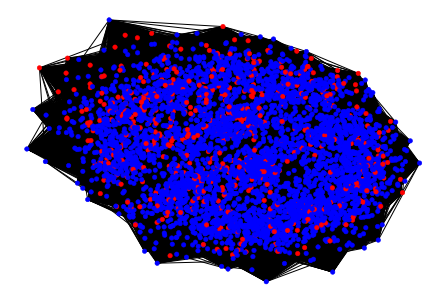
\includegraphics[width=0.7\textwidth]{Moro_network.png}
		\caption{MAG graph of bank telemarketing dataset}
        \label{fig:Moro}
	\end{figure}
  
  \noindent The red dots in figure \ref{fig:Moro} mark the clients which
  decided to invest in the short-term deposit and the blue dots did not invest.
  While this figure masks some of the nodes due to the figure generation
  process, the general pattern becomes apparent. The red nodes appear to be 
  randomly placed in the network which suggests, that the demographic variables 
  which are suitable and were used for the MAG generation process do not
  capture the structure of the label well. The graph further shows, that only a
  relatively small number of clients appear to have invested in the short-term
  deposit. To be more precise, in the dataset only consists of 11.524\% of bank
  clients which invested in the short-term deposit. The dataset is therefore 
  relatively unbalanced which makes the classification task rather difficult. 
  Graph representation learning using Node2Vec did not provide any useful 
  results and the GNNs also performed rather poorly. In particular, GNNs tended
  to classify most clients as non-investors and struggled to accurately
  classify clients which did invest. Due to the unbalanced label data, it was
  loss optimizing to predict most nodes as non-investors rather than learning
  the true observations. This behavior was observed for both graph based
  methods and standard machine learning approaches such as ANN or support
  vector machines (SVM). \\

  \noindent This is part of a larger and common problem in a machine learning 
  setting. Possible remedies might include using loss functions which penalize 
  false classifications harsher than a standard cross entropy loss function. 
  Alternatively one could also reduce the data set by dropping observations
  such that the remaining dataset is balanced. This approach has its own
  problem as dropping a large number of observation discards a lot of
  potentially valuable information. It could also put in question the external
  validity of the model. These comments point to a separate field of research
  and could be interesting for a future project. These approaches were not
  researched in detail and should be taken as suggestions. This thesis will not
  focus on this problem which is why this issue is not further investigated. \\

  \noindent The failure using graph machine learning methods for this dataset
  reveals, that GNNs are not an easy remedy for unbalanced data. Perhaps if the
  network structure provided clusters which corresponded to the labels, GNNs
  could provide superior results. Given the variables available in the dataset
  and the limitations of using the MAG method, this was not possible. In order
  to check, whether network structure could indeed remedy the unbalanced label
  problem, the label was used for the MAG network generation process. Indeed by
  setting the link-affinity probabilities as follows for the label, superior
  results were achieved:

  \[ \Theta_{label} = 
	\begin{pmatrix}
        0.95 & 0.25 \\
		0.25 & 0.95 \\
	\end{pmatrix}
	\] \\
  
  \noindent The resulting graph when considering the label is shown in figure
  \ref{fig:Moro_bias}.

  \begin{figure}[h]
		\centering
		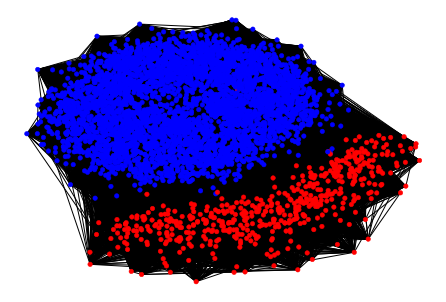
\includegraphics[width=0.7\textwidth]{Moro_network_bias.png}
		\caption{MAG graph of bank telemarketing dataset}
        \label{fig:Moro_bias}
  \end{figure}

  \noindent It now becomes apparent in figure \ref{fig:Moro_bias} that the
  nodes are perfectly separated from each other and grouped according to their
  label. Nevertheless, both node clusters remain connected thanks to the
  stochastic structure of the MAG model. The GNN method GraphSage achieved an 
  accuracy of 100\% for both the training and validation nodes after only 3 
  epochs for the graph shown in figure \ref{fig:Moro_bias}. This is of course a 
  form of cheating, as we cannot assume to know the labels of the entire graph 
  and especially when applying the model to new and unseen data which might not 
  contain any label information. It however shows, that if the graph provides 
  node clusters which corresponds to the node labels, that graph machine 
  learning can overcome the problem of unbalanced data. The difficulty for 
  graph machine learning here is to find graph data including features which 
  naturally captures node clusters which correspond to the node labels. For the 
  synthetic graph generation setting using the MAG model, one would have to
  collect data which generates clusters via the MAG model that highly correlate
  with the label. An example for such a dataset was found and while not
  perfect, it yielded good results and is presented in the following section. 

  \subsection{Airline Passenger Satisfaction Survey}


  \subsection{Stochastic vs. Deterministic MAG}

  As addressed in section \ref{section:self_survey}, the question was raised 
  as to whether the MAG should form connections between observations
  stochastically or whether a deterministic setting yields better results. The 
  first insight gained when investigating this question lies in the fact that 
  the probability of two observations is generally very low. When setting the 
  threshold to 0.5, not a single connection between observations was made. This
  makes sense as the probability of a connection being formed decreases by
  design as the number of generation variables increases. This is implicitly
  shown in equation \ref{eq:MAG} where the product of probabilities is bound to
  decrease. For this reason, it is suggested to set $K=\rho\log_{2}N$
  for some constant $\rho$ \citep[p. 122]{kim2012multiplicative}. For the
  purpose of this thesis, the generation variables were selected such that
  $K\leqslant\log_{2} N$. The airline passenger satisfaction survey was used
  for a deterministic graph generation. The threshold probability for a
  connection was set to 0.2 in the MAG model. The resulting graph consisted of
  several disconnected sub-graphs which were for the most part clustered
  according to their group membership. Figure \ref{fig:det_MAG} shows the
  respective plots of the graph generation variables where the edge connections
  were removed. The sub-graphs are unfortunately small, however all graphs
  combined include all 6'000 nodes. The plots are meant to provide a high-level
  overview of the clusters in the sub-plots. 

  \begin{figure}[h]
		\centering
		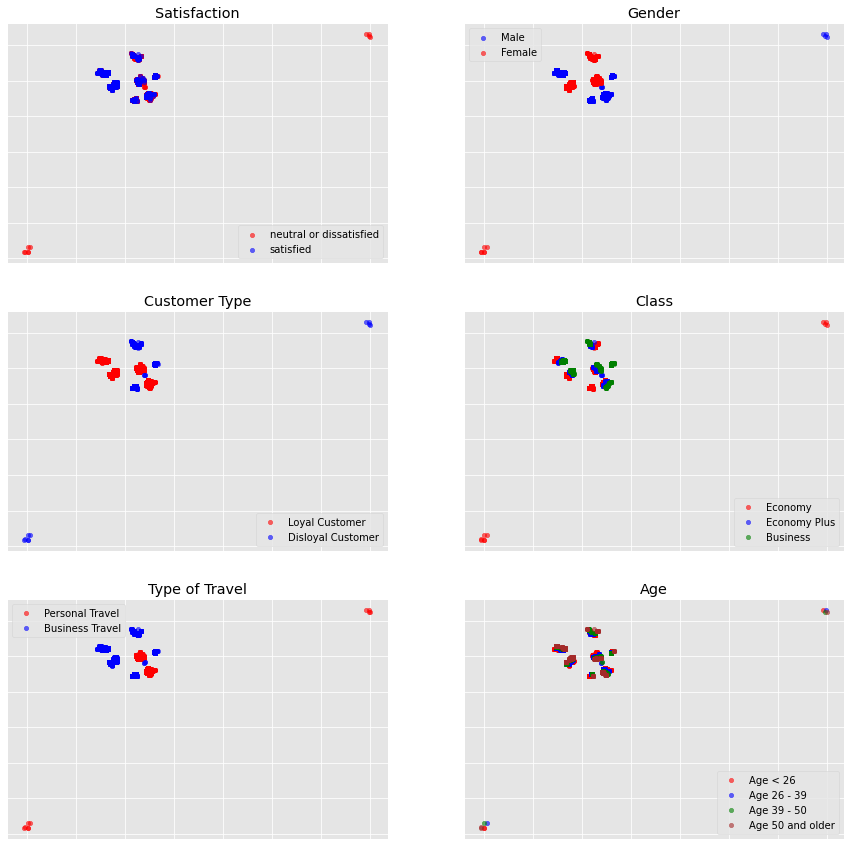
\includegraphics[width=0.7\textwidth]{deterministic_MAG.png}
		\caption{Deterministic MAG graph}
        \label{fig:det_MAG}
  \end{figure}

  \noindent In short, the deterministic graph clustering creates disconnected 
  sub-graphs which forms clusters based on the nodes similarity to each other.
  In terms of performance, the performance and loss behavior of both the
  deterministically and stochastically generated graphs are virtually identical. 
  For the purpose of visualization the stochastically generated graph appears
  to be more useful, as one can identify the different cluster on a single
  connected graph.
  
